\section{Characterisation}

The simulation test bench circuit and set up used in this section were the same as the notes suggests.

\subsection{Gain}

This op amp consists of two gain stages, a differential input stage and an amplification stage.

The differential gain of the long tailed pair (LTP) differential stage can be modelled as:

$$
A_1 = \frac{V_o}{V_{inp} - V_{inn}} = \frac{I_o R_o}{V_d}
    = \frac{2 g_{mp} \times \frac{V_d}{2}}{V_d}(r_{on1} \parallel r_{op1})
    = g_{mp} (r_{on1} \parallel r_{op1})
$$

Where $g_{mp}$ refers to the transconductance of the differential pair PMOS 0 and 1, and $r_{on1}$ and $r_{op1}$ are the output resistances of NMOS1 and PMOS1 respectively.

Using results browser and DC operating points, the $g_m$ and $r_{o}$ parameters of these MOSFETs under saturation can be extracted:

$$ g_{pm} \approx 1.323m S; \qquad r_{on1} \approx 148.5k \Omega; \qquad r_{op1} \approx 110.4k \Omega $$

The gain of the differential stage can be therefore calculated as $A_1 \approx 83.78$.

The second amplification stage is a common source amplifier, using a single NMOS transistor. The gain of this stage is therefore:

$$ A_2 = \frac{V_o}{V_i} = \frac{I_o R_o}{V_i} = g_{mn} (R_{on3} \parallel R_{op4} \parallel R_L) $$

Where $R_{on3}$ and $R_{op4}$ is the output resistances of NMOS3 and PMOS4 respectively, and the load resistance is $R_L = 10k \Omega$. From DC operating point data under saturation:

$$ g_{mn} \approx 5.371m S; \qquad R_{on3} \approx 19.82k \Omega; \qquad R_{op4} \approx 16.50k \Omega $$

So the gain of the amplification stage is $A_2 \approx 25.45$.

Therefore, the overall voltage gain is $A_{OL} = A_1 A_2 \approx 2132$.

This value can then be verified by plotting $V_{OUT}$ against $V_{INP} - V_{INN} = V_d$. For tiny changes of $V_d$ around a specific operating point, the variation of $V_{OUT}$ may be considered as a linear variation, i.e. $A = \frac{\delta V_{OUT}}{\delta V_d}$. Therefore, a DC sweep analysis can be used to evaluate the open loop gain, by plotting the gradient of the transfer curve, then find the maximum value. This can be done by using the \texttt{deriv} calculator function. As shown in Figure \ref{fig:dc_s}, the open loop gain is about $4.302k / 2 = 2.151k$, matches the calculated value. The value was divided by 2 because the horizontal axis of the DC sweep analysis is half the differential voltage input.

As can be seen from the DC sweep analysis, the maxima on the gain curve has a slight offset against the $0 V$ differential voltage. This is mostly due to mismatch of gain and output resistance values of the bottom current mirror and the amplification stage (PMOS4 and NMOS3), resulting in a small input offset voltage. However, the Virtuoso suite only saves operating point when the differential voltage is exactly $0 V$. A small offset voltage of $660\mu V$ was therefore applied to the \texttt{INN} terminal, moving the maxima towards the origin, before extracting MOSFET parameters. This improved the accuracy of gain calculation a lot.

\begin{figure}[!htb]
	\centering
	\begin{subfigure}[b]{0.45\textwidth}
		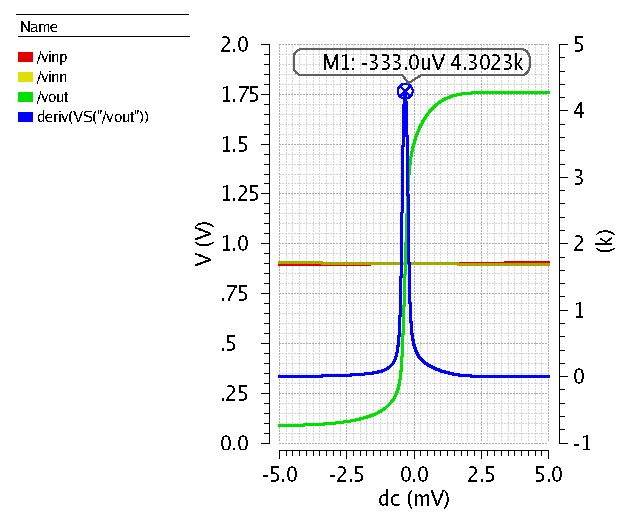
\includegraphics[width=\textwidth]{dc}
		\caption{Overview}
		\label{fig:dc_o}
	\end{subfigure}
	\begin{subfigure}[b]{0.45\textwidth}
		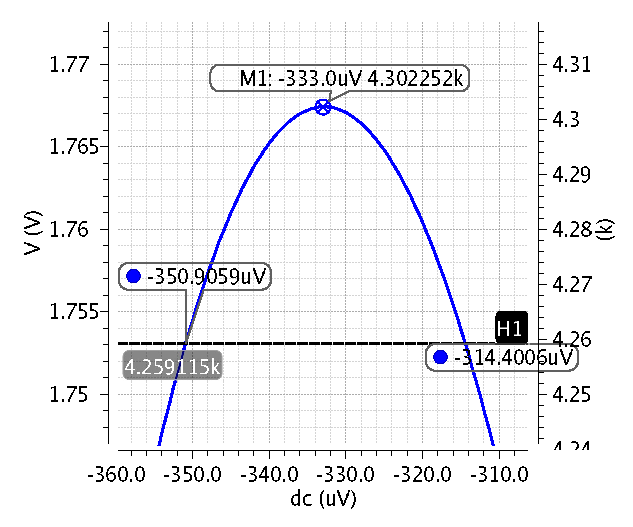
\includegraphics[width=\textwidth]{dc_s}
		\caption{Peak open loop gain}
		\label{fig:dc_s}
	\end{subfigure}
	\caption{DC analysis of the OTA design}
	\label{fig:dc}
\end{figure}

\subsection{Cut-off frequency}

Figure \ref{fig:small} shows a simplified small signal model of the op amp with compensation using Miller effect.

\begin{figure}[!htb]
	\centering
	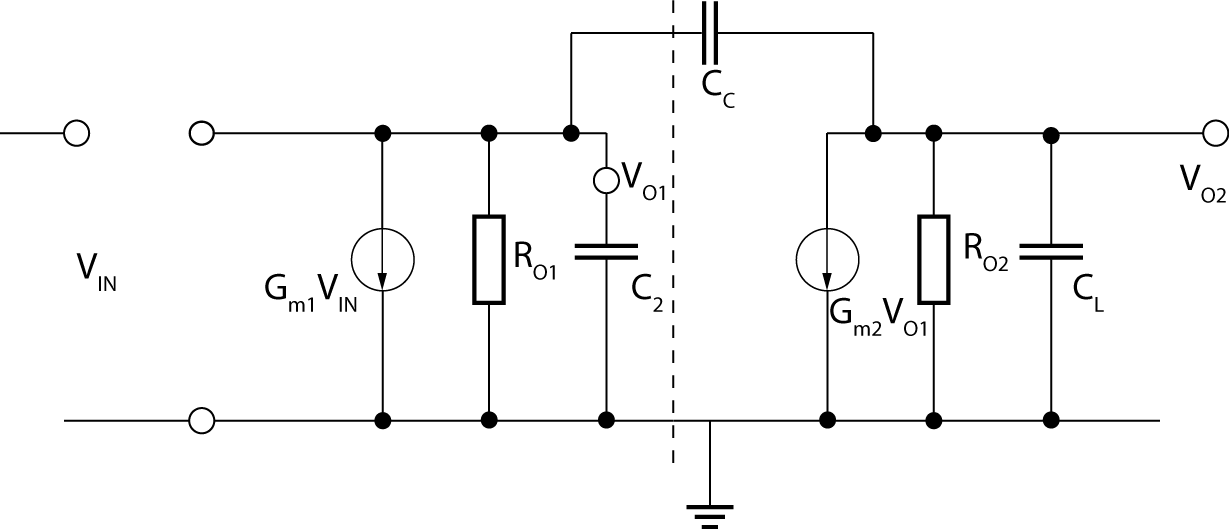
\includegraphics[width=0.8\textwidth]{small}
	\caption{Simplified small signal model of an op amp with compensation}
	\label{fig:small}
\end{figure}

Applying Miller's approximation, the frequency of the dominate pole at low frequency is given by:

$$ fp_1 = \frac{1}{2 \pi G_{m2} R_{o1} R_{o2} C_c} $$

Where $G_{m2}$ is $g_m$ of NMOS3, $R_{o1}$ is $R_{op1} \parallel R_{on1}$, $R_{o2}$ is $R_{on3} \parallel R_{op3} \parallel R_L$, and $C_c = 10 \times 3 \times 104f F$.

Using the numbers from operating point extraction and schematic design, the result is $fp_1 = f_{3dB} \approx 30.22k Hz$.

Together with the open loop gain, these can be used to derive the bandwidth of this op amp, by using the gain-bandwidth product, where

$$ GB = A \times f $$

Therefore, the bandwidth when $\text{gain} = 0$ should be approximately

$$ f_{bw} = \frac{GB}{1} = A_{OL} f_{3dB} \approx 65.0 MHz $$

By doing an AC analysis with the loads, the bandwidth can be evaluated as shown in Figure \ref{fig:ac}.

\begin{figure}[!htb]
	\centering
	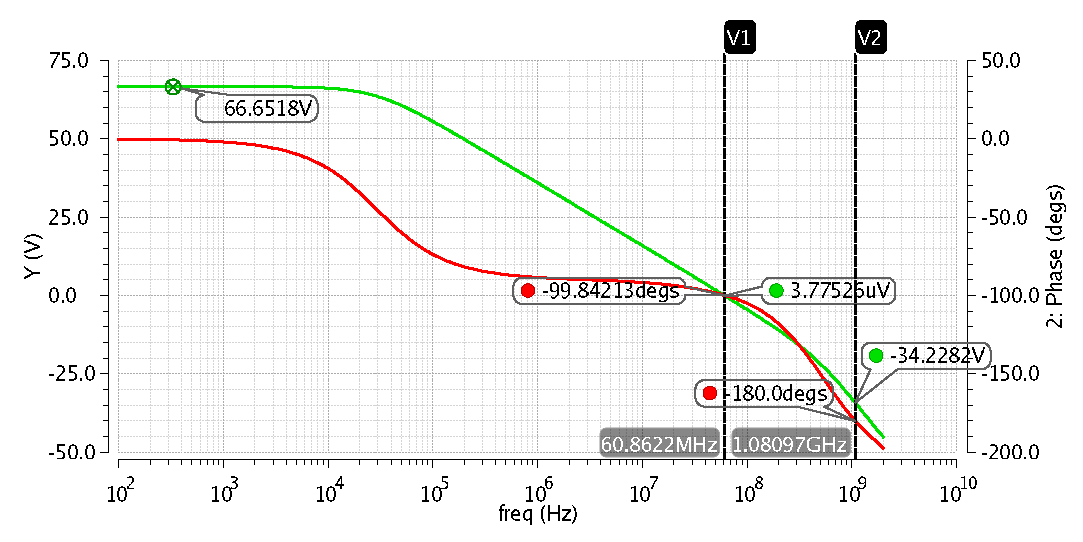
\includegraphics[width=0.8\textwidth]{ac}
	\caption{AC analysis of the op amp}
	\label{fig:ac}
\end{figure}

The bandwidth value from simulation is about $60.9M Hz$ at marker V1, matches the calculation.

\subsection{Linear input range}

The linear input range is defined as the range when transconductance of the op amp reduced by $1\%$. Assuming constant output resistance, this will result in the open loop voltage gain reduced by $1\%$, which is shown in the DC sweep analysis (Figure \ref{fig:dc_s}).

As the horizontal axis is half the differential voltage, the linear range should be from $-350.9\mu V \times 2 = -701.8\mu V$ to $314.4\mu V \times 2 = -628.8\mu V$, about $73\mu V$. This is a very limited range, but since the op amp has a very large gain, and typically works in a feedback configuration, having a non-linear input characteristic will not cause a significant problem.

\subsection{Gain improvements}

The overall gain of this op amp can be improved by increasing the transconductance $g_m$ of some transistors, including PMOS0 and PMOS1 in the differential pair configuration, NMOS3 and PMOS4 in the amplification stage.

According to MOSFET modelling equation (Equation \ref{eq:mosgm}), for a given technology (i.e. constant doping concentration, gate oxide capacitance, etc.), the transconductance may be improved by increasing $\frac{W}{L}$ ratio. For analogue design, it is preferred to increase the gate length, but not decrease gate width, to avoid device mismatch issues. Increasing the supply voltage, which will in turn increase $V_{GS}$, may also increase the gain of the amplifier.

\begin{align}
	g_m = \mu_n C_{ox} \frac{W}{L} (V_{GS} - V_{TH})
	\label{eq:mosgm}
\end{align}

\subsection{Slew rate}

Slew rate is defined as the maximum output swing speed the amplifier can achieve, i.e. $SR = \max(\frac{\Delta V}{\Delta t})$.

For this op amp, it can be evaluated as:

$$ SR = \max(\frac{\Delta V}{\Delta t}) = <max(\frac{i_c}{C_L}) $$

Biasing current determines the maximum current ($i_c$) the amplifier can output to drive capacitive loads ($C_L$). It is proportional to the slew rate, according to the equation. The biasing currents for PMOS4 and NMOS3 determines the slew rate for output rising and falling respectively.

Figure \ref{fig:trans_s} shows a rising edge of the amplifier output from transient analysis. The delta marker shows the gradient of the rising output, about $68.2 MV/s$, is the slew rate of the op amp.

\begin{figure}[!htb]
	\centering
	\begin{subfigure}[b]{0.45\textwidth}
		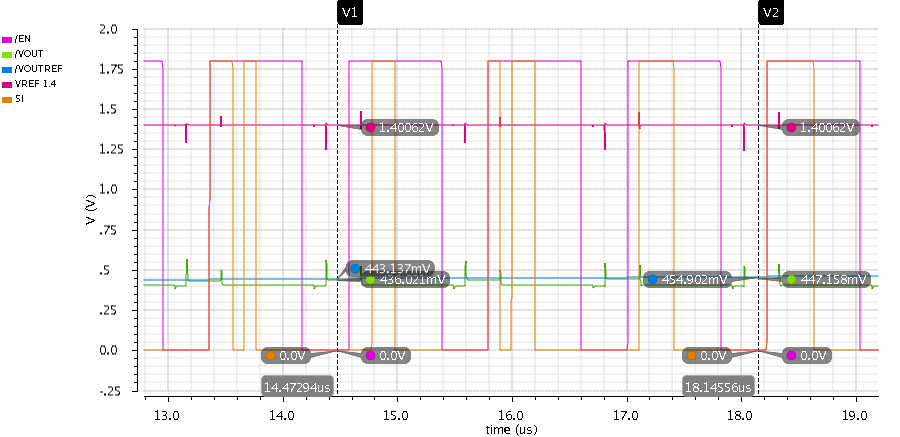
\includegraphics[width=\textwidth]{trans}
		\caption{Overview}
		\label{fig:trans_o}
	\end{subfigure}
	\begin{subfigure}[b]{0.45\textwidth}
		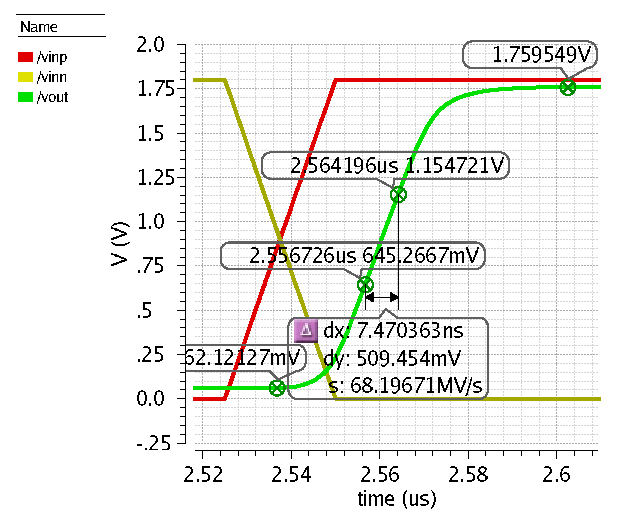
\includegraphics[width=\textwidth]{trans_s}
		\caption{Output rising edge}
		\label{fig:trans_s}
	\end{subfigure}
	\caption{Transient analysis of the OTA design}
\end{figure}
